\documentclass{article}
\usepackage{graphicx} % Required for inserting images
\usepackage{titlesec}
\usepackage{float}
\usepackage{listings}
\usepackage{enumitem}
\usepackage[top=1in, bottom=1in, left=1.25in, right=1.25in]{geometry}
\usepackage{amsmath}
\usepackage{tikz}
\usetikzlibrary{positioning}
% Configure section numbering
\renewcommand{\thesection}{Part \Alph{section}}
\renewcommand{\thesubsection}{\arabic{subsection}:}
\renewcommand{\thesubsubsection}{(\alph{subsubsection})}


% Adjust section format
\titleformat{\section}{\normalfont\Large\bfseries}{\thesection}{1em}{}
\titleformat{\subsection}{\normalfont\large\bfseries}{\thesubsection}{1em}{}
\titleformat{\subsubsection}{\normalfont\normalsize\bfseries}{\thesubsubsection}{1em}{}


\title{\textbf{COL759 Cryptography and Computer Security Assignment 2}}
\author{Anshik Sahu(2021CS10577) \& Sanya Mittal(2021CS10565)}
\date{September 2023}

\begin{document}

\maketitle
\tableofcontents
\newpage
\section{}
\subsection{Cryptosystems secure against side-channel attacks}
Given : F : $\{0,1\}^n$ × $\{0,1\}^n$ → $\{0,1\}^n$, a secure PRF. \\
Goal: To construct a secure PRF F' where leaking one bit of the key breaks PRF security. \\ \\ 
Let the Key Space of F', K' = $\{0,1\}^{n+1}$, input space X' = $\{0,1\}^n$ and output space Y' = $\{0,1\}^n$. \\
Let $k \in \{0,1\}^n$ and $b \in \{0,1\}$.
 \\

$$ F'(k_1 = k \| b,x) = 
    \begin{cases}
      {F(k,x)}, & \text{if}\ {x \neq 0^n}\\
      {b\|\ F(k,x)[1:]}, & \text{otherwise}
    \end{cases} $$

\subsubsection{Proof by Contra-positive}
We prove the security of F' by showing that if there exists an adversary A that can distinguish the output of F'(k,.) for a uniformly randomly sampled key k from a truly random function f(.) with some non-negligible advantage, then there exists an adversary that can distinguish the output of F(k,.) for a uniformly randomly sampled key k from a truly random function f(.) with some non-negligible advantage. \\ \\ \\

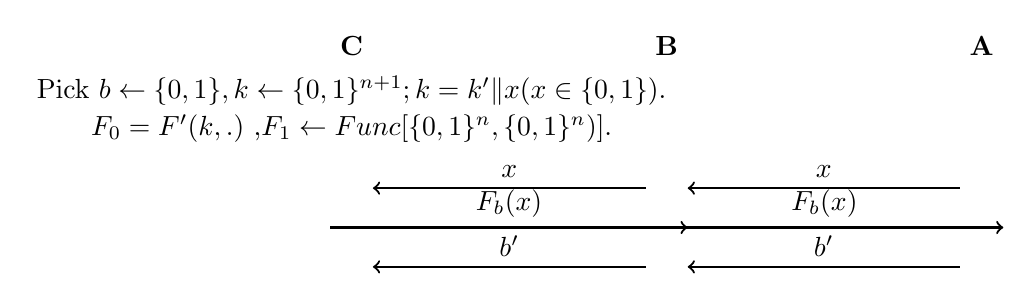
\begin{tikzpicture}
    % Nodes
    \node (challenger) at (0,0) {\textbf{C}};
    \node (bob) at (4,0) {\textbf{B}};
    \node (adversary) at (8,0) {\textbf{A}};
    
    \node[below=0.001cm of challenger] {Pick $b\leftarrow\{0,1\}, k\leftarrow\{0,1\}^{n+1}; k = k' \| x ( x \in \{0,1\}) $.};
    \node[below=0.5cm of challenger]{ $F_0= F'(k,.)$ ,$F_1\leftarrow Func[\{0,1\}^{n},\{0,1\}^{n})]$.};

    
    
    
    % Arrows
    \draw[->, thick] ([yshift=-1.8cm]adversary.west) -- node[above] {$x$} ([yshift=-1.8cm]bob.east);
    \draw[->, thick] ([yshift=-1.8cm]bob.west) -- node[above] {$x$} ([yshift=-1.8cm]challenger.east);
    \draw[->, thick] ([yshift=-2.3cm]challenger.west) -- node[above] {$F_b(x)$} ([yshift=-2.3cm]bob.east);
    \draw[->, thick] ([yshift=-2.3cm]bob.west) -- node[above] {$F_b(x)$} ([yshift=-2.3cm]adversary.east);
    \draw[->, thick] ([yshift=-2.8cm]adversary.west) -- node[above] {$b'$} ([yshift=-2.8cm]bob.east);
    \draw[->, thick] ([yshift=-2.8cm]bob.west) -- node[above] {$b'$} ([yshift=-2.8cm]challenger.east);
\end{tikzpicture}
\\ \\
Let Adversary A can distinguish the output of F'(k,.) for a uniformly randomly sampled key k from a truly random function f(.) with probability $\frac{1}{2}$ + $\epsilon$. \\
\[
\begin{aligned}
    &\text{Pr}[B \text{ wins }] = \text{Pr}[ B \text{ wins } \land x = 0^n] +  \text{Pr}[ B \text{ wins } \land x \neq 0^n] \\ \\
    &\text{When } x \neq 0^n  \text{adversary gets F(k,x),so adversary can distinguish with a probability } \frac{1}{2} + \epsilon \text{ as it is the} \\
    &\text{same as playing against PRF Challenger of F}. \\ \\
    &\text{And when x= $0^n$, even if the adversary has no advantage in guessing b, it can still make a random} \\
    &\text{guess with a probability of $\frac{1}{2}$ } \\
    &\text{ Thus probability of B winning in this case is atleast 1/2 (random guess).} \\
    &\text{Pr}[B \text{ wins }] >= (1- \frac{1}{2^n}) * (\frac{1}{2} + \epsilon) +  \frac{1}{2^n} * \frac{1}{2} = \frac{1}{2} + \epsilon* (1-\frac{1}{2^n}) \\
    &\text{Thus the adversary has a non-negligible advantage of winning. Thus, by PRF Security of F, F' is a} \\
    &\text{secure PRF. }
\end{aligned}
\]


\subsubsection{F' does not satisfy 1-leakage resilience.}

Goal : To construct a PPT Adversary A that wins the Security Game for Leakage resilient PRFs with non-negligible advantage. \\
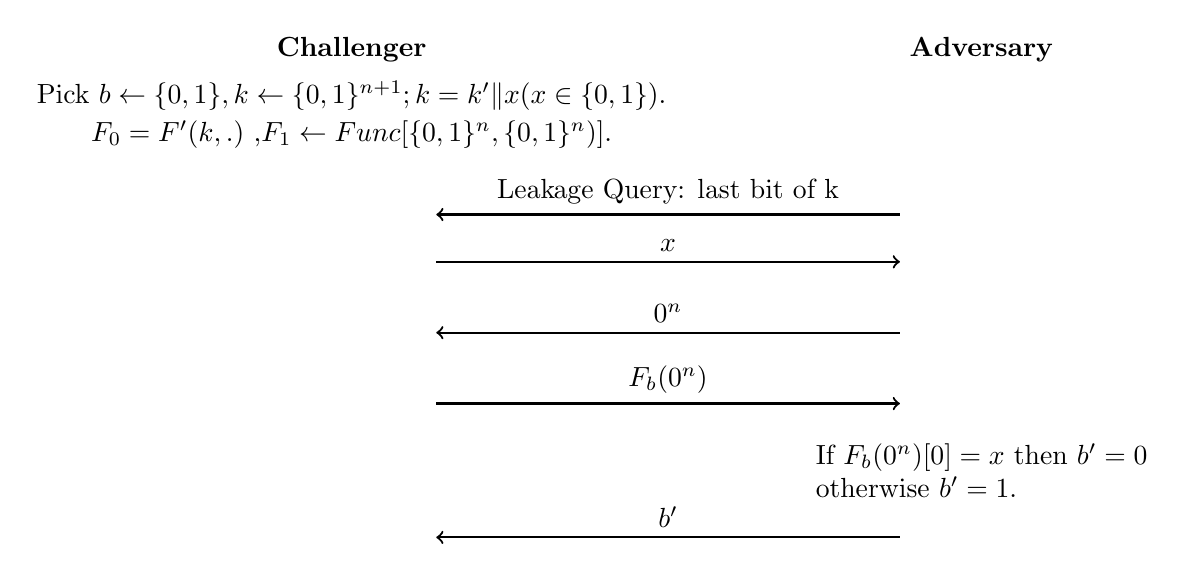
\begin{tikzpicture}
    % Nodes
    \node (challenger) at (0,0) {\textbf{Challenger}};
    \node (adversary) at (8,0) {\textbf{Adversary}};
    \node[below=0.001cm of challenger] {Pick $b\leftarrow\{0,1\}, k\leftarrow\{0,1\}^{n+1}; k = k' \| x ( x \in \{0,1\}) $.};
    \node[below=0.5cm of challenger]{ $F_0= F'(k,.)$ ,$F_1\leftarrow Func[\{0,1\}^{n},\{0,1\}^{n})]$.};

    \node [align= justify, below = 4.6cm of adversary] {If $F_b(0^n)[0]=x$ then $b'=0$ \\ otherwise $b'=1$.};
    
    % Arrows
    \draw[->, thick] ([yshift=-2.1cm]adversary.west) -- node[above] {Leakage Query: last bit of k} ([yshift=-2.1cm]challenger.east);    
    \draw[->, thick] ([yshift=-2.7cm]challenger.east) -- node[above] {$x$} ([yshift=-2.7cm]adversary.west);

    \draw[->, thick] ([yshift=-3.6cm]adversary.west) -- node[above] {$0^n$} ([yshift=-3.6cm]challenger.east);    
    \draw[->, thick] ([yshift=-4.5cm]challenger.east) -- node[above] {$F_b(0^n)$} ([yshift=-4.5cm]adversary.west);
    \draw[->, thick] ([yshift=-6.2cm]adversary.west) -- node[above] {$b'$} ([yshift=-6.2cm]challenger.east);
\end{tikzpicture} \\ \\ \\

Advantage of this adversary = $\Pr[A \text{ outputs } 0 \,|\, C \text{ chooses } 0] - \Pr[A \text{ outputs } 0 \,|\, C \text{ chooses } 1]$ \\ \\
$\Pr[A \text{ outputs } 0 \,|\, C \text{ chooses } 0]$ = $\Pr[\text{$0^{th}$ bit of y= }x |\ F_b \text{ is a PRF}] = 1$ \\
$\Pr[A \text{ outputs } 0 \,|\, C \text{ chooses } 1]$ = $\Pr[\text{$0^{th}$ bit of y= }x |\ F_b \text{ is } \text{a uniformly random function}] = \frac{1}{2}$ \\
Advantage of A $ \approx 1 - \frac{1}{2} = \frac{1}{2}$ \\
Thus, $Pr[A wins the 1-leakage resilience game] \approx \frac{1}{2} + \frac{1}{2}*\frac{1}{2} \approx \frac{3}{4}$

\newpage
\subsection{MACs: unique queries vs non-unique queries}
\subsubsection{MAC Scheme}
Given a pseudorandom function $F: \{0,1\}^n \times \{0,1\}^n \rightarrow \{0,1\}^n $,
the Signing Algorithm samples randomness $r_0$ and $r_1$ from $\{0,1\}^{n-4}$ and a key $k$ from $\{0,1\}^{n}$.
\[Sign(k,m)=a||b\text{ , where}\]
\[a=r_0\big|\big| F(k,m[0:\lceil n/2 \rceil ]\big|\big|00\big|\big|r_0[0:\lfloor n/2 \rfloor -2])\big|\big|F(k,m[\lceil n/2 \rceil:n ]\big|\big|01\big|\big|r_0[\lfloor n/2 \rfloor -2:n-4])\]
\[b=r_1\big|\big|F(k,m[0:\lceil n/2 \rceil ]\big|\big|10\big|\big|r_1[0:\lfloor n/2 \rfloor -2])\big|\big|F(k,m[\lceil n/2 \rceil:n ]\big|\big|11\big|\big|r_1[\lfloor n/2 \rfloor -2:n-4])\]
\\
\[Verify(k,m,a||b)=\begin{cases} 1 & \text{if } check(k,m,a)=check(k,m,b)=1\\
0 & \text{otherwise}\end{cases}\text{ , where}\]
\[check(k,m,x)=\begin{cases}1 & \text{if }\\&x=r\big|\big| F(k,m[0:\lceil n/2 \rceil ]\big|\big|00\big|\big|r[0:\lfloor n/2 \rfloor -2])\big|\big|F(k,m[\lceil n/2 \rceil:n ]\big|\big|01\big|\big|r[\lfloor n/2 \rfloor -2:n-4])\\&where, r=x[0:n-4]\\
0 & \text{otherwise}\end{cases}\]
Here, $x[a:b]$ means $x$ from index $a$ to $b$, including $x[a]$ but excluding $x[b]$.

\subsubsection{UFCMA-Unique security}
To prove the security UFCMA security of the scheme, we create the following hybrid worlds:
Note: In each world, the challenger also chooses a key.
\begin{itemize}
        \item World 0: 
        \begin{itemize}
            \item Challenger receives new m.
            \item Challenger chooses $r_0$ and $r_1$ from $\{0,1\}^{n-4}$.
            \item Challenger sends $a||b$ , where
\[a=r_0\big|\big| F(k,m[0:\lceil n/2 \rceil ]\big|\big|00\big|\big|r_0[0:\lfloor n/2 \rfloor -2])\big|\big|F(k,m[\lceil n/2 \rceil:n ]\big|\big|01\big|\big|r_0[\lfloor n/2 \rfloor -2:n-4])\]
\[b=r_1\big|\big|F(k,m[0:\lceil n/2 \rceil ]\big|\big|10\big|\big|r_1[0:\lfloor n/2 \rfloor -2])\big|\big|F(k,m[\lceil n/2 \rceil:n ]\big|\big|11\big|\big|r_1[\lfloor n/2 \rfloor -2:n-4])\]
            \item A outputs b'.
            \[Pr[A \text{ outputs }0]=p_0\]
        \end{itemize}
        \item Hybrid World 1:
        \begin{itemize}
            \item Challenger receives new m.
            \item Challenger chooses $r_0$ and $r_1$ from $\{0,1\}^{n-4}$ and $p$ from $\{0,1\}^{n}$.
            \item Challenger sends $a||b$ , where
\[a=r_0\big|\big|p\big|\big|F(k,m[\lceil n/2 \rceil:n ]\big|\big|01\big|\big|r_0[\lfloor n/2 \rfloor -2:n-4])\]
\[b=r_1\big|\big|F(k,m[0:\lceil n/2 \rceil ]\big|\big|10\big|\big|r_1[0:\lfloor n/2 \rfloor -2])\big|\big|F(k,m[\lceil n/2 \rceil:n ]\big|\big|11\big|\big|r_1[\lfloor n/2 \rfloor -2:n-4])\]
            \item A outputs b'.
            \[Pr[A \text{ outputs }0]=p_{H1}\]
        \end{itemize}
        \item Hybrid World 2:
        \begin{itemize}
            \item Challenger receives new m.
            \item Challenger chooses $r_0$ and $r_1$ from $\{0,1\}^{n-4}$ and $p$ and $q$ from $\{0,1\}^{n}$.
            \item Challenger sends $a||b$ , where
\[a=r_0\big|\big|p\big|\big|q\]
\[b=r_1\big|\big|F(k,m[0:\lceil n/2 \rceil ]\big|\big|10\big|\big|r_1[0:\lfloor n/2 \rfloor -2])\big|\big|F(k,m[\lceil n/2 \rceil:n ]\big|\big|11\big|\big|r_1[\lfloor n/2 \rfloor -2:n-4])\]
            \item A outputs b'.
            \[Pr[A \text{ outputs }0]=p_{H2}\]
        \end{itemize}
        \item Hybrid World 3:
        \begin{itemize}
            \item Challenger receives new m.
            \item Challenger chooses $r_0$ and $r_1$ from $\{0,1\}^{n-4}$ and $p$, $q$ and $r$ from $\{0,1\}^{n}$.
            \item Challenger sends $a||b$ , where
\[a=r_0\big|\big|p\big|\big|q\]
\[b=r_1\big|\big|r\big|\big|F(k,m[\lceil n/2 \rceil:n ]\big|\big|11\big|\big|r_1[\lfloor n/2 \rfloor -2:n-4])\]
            \item A outputs b'.
            \[Pr[A \text{ outputs }0]=p_{H3}\]
        \end{itemize}
        \item World 1: 
        \begin{itemize}
            \item Challenger receives new m.
            \item Challenger chooses $r_0$ and $r_1$ from $\{0,1\}^{n-4}$ and $p$, $q$, $r$ and $s$ from $\{0,1\}^{n}$.
            \item Challenger sends $a||b$ , where
\[a=r_0\big|\big|p\big|\big|q\]
\[b=r_1\big|\big|r\big|\big|s\]
            \item A outputs b'.
            \[Pr[A \text{ outputs }0]=p_{1}\]
        \end{itemize}
    \end{itemize}
\textbf{Proof by contrapositive}\\
Let there be a ppt. adversary A, which breaks the UFCMA-Unique security of the scheme. Thus,
\[|p_0-p_1|\text{ is non-negligible.}\]
From this, we can imply at least one from $|p_0-p_{H1}$, $|p_{H1}-p_{H2}$, $|p_{H2}-p_{H3}$, $|p_{H3}-p_1$ is non-negligible.\\
We can define a set of reductions $B_i$ each of the following form:
\begin{figure}[H]
    \centering
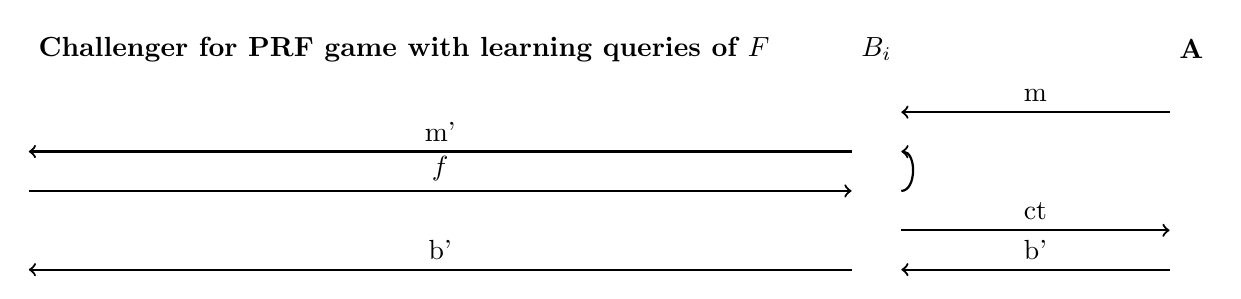
\begin{tikzpicture}
    % Nodes
    \node (challenger) at (0,0) {\textbf{Challenger for PRF game with learning queries of \(F\)}};
    \node (bob) at (6,0) {\textbf{\(B_i\)}};
    \node (adversary) at (10,0) {\textbf{A}};
    % Arrows
    \draw[->, thick] ([yshift=-0.8cm]adversary.west) -- node[above] {m} ([yshift=-0.8cm]bob.east);
    \draw[->, thick] ([yshift=-1.3cm]bob.west) -- node[above] {m'} ([yshift=-1.3cm]challenger.west);
    \draw[->, thick] ([yshift=-1.8cm]challenger.west) -- node[above] {\(f\)} ([yshift=-1.8cm]bob.west);
    % Curved arrow for repetition
    \draw[->, thick] ([yshift=-1.8cm]bob.east) to[out=1,in=-1] node[below] {} ([yshift=-1.3cm]bob.east);
    \draw[->, thick] ([yshift=-2.3cm]bob.east) -- node[above] {ct} ([yshift=-2.3cm]adversary.west);
    \draw[->, thick] ([yshift=-2.8cm]adversary.west) -- node[above] {b'} ([yshift=-2.8cm]bob.east);
    \draw[->, thick] ([yshift=-2.8cm]bob.west) -- node[above] {b'} ([yshift=-2.8cm]challenger.west);
\end{tikzpicture}
\end{figure}
\begin{itemize}
    \item $B_1$
    \begin{itemize}
        \item Receives m from A.
        \item chooses $r_0$ and $r_1$ from $\{0,1\}^{n-4}$
        \item Sends learning queries for a,b,c to the challenger, where
        \[a=m[\lceil n/2 \rceil:n ]\big|\big|01\big|\big|r_0[\lfloor n/2 \rfloor -2:n-4]\]
        \[b=m[0:\lceil n/2 \rceil ]\big|\big|10\big|\big|r_1[0:\lfloor n/2 \rfloor -2]\]
        \[c=m[\lceil n/2 \rceil:n ]\big|\big|11\big|\big|r_1[\lfloor n/2 \rfloor -2:n-4]\]
        \item Receives $ct_1$, $ct_2$ and $ct_3$ respectively.
        \item Sends query for m'=$m[0:\lceil n/2 \rceil ]\big|\big|00\big|\big|r_0[0:\lfloor n/2 \rfloor -2]$ to the challenger and receives $ct_0$.
        \item Sends $r_0||ct_0||ct_1||r_1||ct_2||ct_3$ to A and receives b'.
        \item Sends b' as its guess to challenger.
    \end{itemize}
    If $|p_0-p_{H1}|$ is non-negligible, A can distinguish between World 0 and Hybrid World 1. If Challenger chooses $b=0$, this is equivalent to World 0 and if challenger chooses $b=1$, this is equivalent to Hybrid world 1. Thus by construction, $B_1$ breaks the security of $F$
    \item $B_2$
    \begin{itemize}
        \item Receives m from A.
        \item chooses $r_0$ and $r_1$ from $\{0,1\}^{n-4}$
        \item chooses $ct_0$ from $\{0,1\}^n$
        \item Sends learning queries for b,c to the challenger, where
        \[b=m[0:\lceil n/2 \rceil ]\big|\big|10\big|\big|r_1[0:\lfloor n/2 \rfloor -2]\]
        \[c=m[\lceil n/2 \rceil:n ]\big|\big|11\big|\big|r_1[\lfloor n/2 \rfloor -2:n-4]\]
        \item Receives $ct_2$ and $ct_3$ respectively.
        \item Sends query for m'=$m[\lceil n/2 \rceil:n ]\big|\big|01\big|\big|r_0[\lfloor n/2 \rfloor -2:n-4]$ to the challenger and receives $ct_1$.
        \item Sends $r_0||ct_0||ct_1||r_1||ct_2||ct_3$ to A and receives b'.
        \item Sends b' as its guess to challenger.
    \end{itemize}
    If $|p_{H1}-p_{H2}|$ is non-negligible, A can distinguish between Hybrid World 1 and Hybrid World 2. If Challenger chooses $b=0$, this is equivalent to Hybrid World 1 and if challenger chooses $b=1$, this is equivalent to Hybrid world 2. Thus by construction, $B_2$ breaks the security of $F$
    \item $B_3$
    \begin{itemize}
        \item Receives m from A.
        \item chooses $r_0$ and $r_1$ from $\{0,1\}^{n-4}$
        \item chooses $ct_0$ and $ct_1$ from $\{0,1\}^n$
        \item Sends learning queries for c to the challenger, where
        \[c=m[\lceil n/2 \rceil:n ]\big|\big|11\big|\big|r_1[\lfloor n/2 \rfloor -2:n-4]\]
        \item Receives $ct_3$.
        \item Sends query for m'=$m[0:\lceil n/2 \rceil ]\big|\big|10\big|\big|r_1[0:\lfloor n/2 \rfloor -2]$ to the challenger and receives $ct_2$.
        \item Sends $r_0||ct_0||ct_1||r_1||ct_2||ct_3$ to A and receives b'.
        \item Sends b' as its guess to challenger.
    \end{itemize}
    If $|p_{H2}-p_{H3}|$ is non-negligible, A can distinguish between Hybrid World 2 and Hybrid World 3. If Challenger chooses $b=0$, this is equivalent to Hybrid World 2 and if challenger chooses $b=1$, this is equivalent to Hybrid world 3. Thus by construction, $B_3$ breaks the security of $F$
    \item $B_4$
    \begin{itemize}
        \item Receives m from A.
        \item chooses $r_0$ and $r_1$ from $\{0,1\}^{n-4}$
        \item chooses $ct_0$, $ct_1$ and $ct_2$ from $\{0,1\}^n$
        \item Sends query for m'=$m[\lceil n/2 \rceil:n ]\big|\big|11\big|\big|r_1[\lfloor n/2 \rfloor -2:n-4]$ to the challenger and receives $ct_3$.
        \item Sends $r_0||ct_0||ct_1||r_1||ct_2||ct_3$ to A and receives b'.
        \item Sends b' as its guess to challenger.
    \end{itemize}
    If $|p_{H3}-p_1|$ is non-negligible, A can distinguish between Hybrid World 3 and World 1. If Challenger chooses $b=0$, this is equivalent to Hybrid World 3 and if challenger chooses $b=1$, this is equivalent to World 1. Thus by construction, $B_4$ breaks the security of $F$
\end{itemize}

Thus, for an adversary A which breaks the scheme, using $B_1$, $B_2$, $B_2$, $B_3$ and A, we can define a reduction B, which randomly chooses between $B_1$, $B_2$, $B_2$ and $B_3$. Thus, it has $\frac{1}{4}$ chance of choosing the correct reduction which breaks $F$. Hence, the probability that B breaks the security of $F$ is non-negligible.

Thus, if this scheme is not secure, $F$ is also not secure. Thus, from $F$ being secure PRF, the scheme is UFCMA-unique secure.

\subsubsection{UFCMA security}
To show that the scheme is not UFCMA secure, we define the following adversary A:
\begin{figure}[H]
    \centering
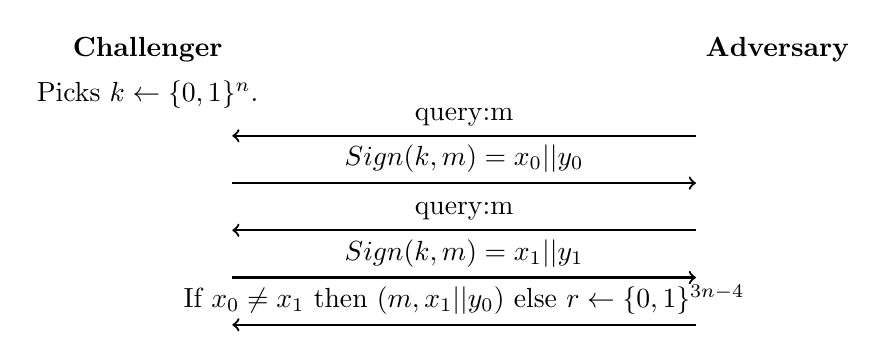
\begin{tikzpicture}
    % Nodes
    \node (challenger) at (0,0) {\textbf{Challenger}};
    \node (adversary) at (8,0) {\textbf{Adversary}};
    \node[below=0.001cm of challenger] {Picks $ k\leftarrow\{0,1\}^{n}$.};    
    % Arrows
    \draw[->, thick] ([yshift=-1.1cm]adversary.west) -- node[above] {query:m} ([yshift=-1.1cm]challenger.east);    
    \draw[->, thick] ([yshift=-1.7cm]challenger.east) -- node[above] {$Sign(k,m)=x_0||y_0$} ([yshift=-1.7cm]adversary.west);

    \draw[->, thick] ([yshift=-2.3cm]adversary.west) -- node[above] {query:m} ([yshift=-2.3cm]challenger.east);    
    \draw[->, thick] ([yshift=-2.9cm]challenger.east) -- node[above] {$Sign(k,m)=x_1||y_1$} ([yshift=-2.9cm]adversary.west);
    \draw[->, thick] ([yshift=-3.5cm]adversary.west) -- node[above] {If $x_0\neq x_1$ then $(m,x_1||y_0)$ else $r\leftarrow\{0,1\}^{3n-4}$} ([yshift=-3.5cm]challenger.east);
\end{tikzpicture}
\end{figure}
By the construction of the MAC scheme, if $x_0$ is not equal to $x_1$, we can create a new signature for the message $m$ by concatenating either $x_0$ with $y_1$ or $x_1$ with $y_0$. As $x_0$ is not equal to $x_1$, these are different from $x_0||y_0$ and $x_1||y_1$. As the check function for each of $x_0$,$x_1$,$y_0$ and $y_1$ equals 1, $Verify(x_0||y_1)$ and $Verify(x_1||y_0)$ are both 1. Thus,
\[Pr[A wins]=Pr[\text{A wins }| x_0\neq x_1]\times Pr[x_0\neq x_1] + Pr[\text{A wins }|x_0=x_1]\times Pr[x_0=x_1]\]
\[=1\times(1-\frac{1}{2^{n-4}})+(\frac{1}{2^{3n-4}})\times(\frac{1}{2^{n-4}})\]
\[\text{Thus, }Pr[\text{A wins}]\approx 1\text{ , given n is large.}\]
\newpage
\subsection{A mistake in the lecture notes}
Let A be an adversary that runs in time t, makes qs signing queries, qv verification queries, and wins the security game - Unforgeability under Chosen Message Attack with Verification Queries with probability 1. \\
We need to show that the reduction B (which plays the Unforgeability under Chosen Message Attack game without verification queries and upon receiving a verification query (m,$\sigma$) from the adversary, it sends m to the challenger, and receives a signature $\sigma$', if $\sigma$ = $\sigma$', then it sends 1, else it sends 0) does not win with probability 1.
\begin{figure}[H]
    \centering
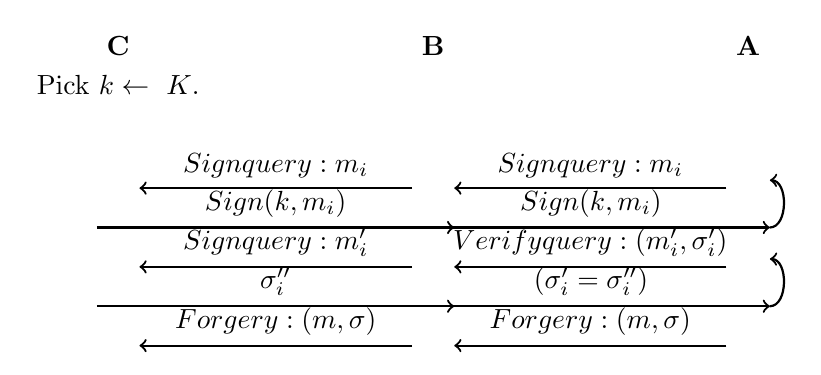
\begin{tikzpicture}
    % Nodes
    \node (challenger) at (0,0) {\textbf{C}};
    \node (bob) at (4,0) {\textbf{B}};
    \node (adversary) at (8,0) {\textbf{A}};
    \node[below=0.001cm of challenger] {Pick  $k\leftarrow\ K$.};
    % Arrows
    \draw[->, thick] ([yshift=-1.8cm]adversary.west) -- node[above] {$Sign query: m_i$} ([yshift=-1.8cm]bob.east);
    \draw[->, thick] ([yshift=-1.8cm]bob.west) -- node[above] {$Sign query: m_i$} ([yshift=-1.8cm]challenger.east);
    \draw[->, thick] ([yshift=-2.3cm]challenger.west) -- node[above] {$Sign(k,m_i)$} ([yshift=-2.3cm]bob.east);
    \draw[->, thick] ([yshift=-2.3cm]bob.west) -- node[above] {$Sign(k,m_i)$} ([yshift=-2.3cm]adversary.east);
    
        \draw[->, thick] ([yshift=-2.3cm]adversary.east) to[out=1,in=-1] node[below] {} ([yshift=-1.7cm]adversary.east);
        \draw[->, thick] ([yshift=-3.3cm]adversary.east) to[out=1,in=-1] node[below] {} ([yshift=-2.7cm]adversary.east);
        
    \draw[->, thick] ([yshift=-2.8cm]adversary.west) -- node[above] {$Verify query: (m'_i,\sigma'_i)$} ([yshift=-2.8cm]bob.east);
    \draw[->, thick] ([yshift=-2.8cm]bob.west) -- node[above] {$Sign query: m'_i$} ([yshift=-2.8cm]challenger.east);
    \draw[->, thick] ([yshift=-3.3cm]challenger.west) -- node[above] {$\sigma_i''$} ([yshift=-3.3cm]bob.east);
    \draw[->, thick] ([yshift=-3.3cm]bob.west) -- node[above] {$(\sigma_i'=\sigma_i'')$} ([yshift=-3.3cm]adversary.east);
    \draw[->, thick] ([yshift=-3.8cm]adversary.west) -- node[above] {$Forgery: (m,\sigma)$} ([yshift=-3.8cm]bob.east);
    \draw[->, thick] ([yshift=-3.8cm]bob.west) -- node[above] {$Forgery: (m,\sigma)$} ([yshift=-3.8cm]challenger.east);
\end{tikzpicture}
\end{figure}
Key Observation: Forgery - adversary sends a message m∗ together with a signature $\sigma$*, and wins if (m*, $\sigma$*) $\neq$ ($m_i$, $\sigma_i$) for all i, and Verify(m*, $\sigma$*, k) = 1. \\ \\
The intuition for such an adversary A is that the adversary can send a verified ($m$, $\sigma$) pair but not a signed pair. Thus A can get queries verified and send them as forgery while reduction B will not be able to send that (m, $\sigma$) pair as forgery.  \\ \\
When Adversary A plays the game with Verification queries, it makes $|K|$ queries to challenger, for a message $m'_i$ and its sign $\sigma'_i$ computed for each key in the Key Space. Since each message has a unique valid signature there will only be one such sigma for which the Verify output is 1, A sends that (m,$\sigma$) pair as forgery and wins with probability 1. Thus $q_v=|K|$, A runs in time t and makes no sign queries.\\ \\
The reduction B, for each verification query, will send m to the challenger and it will send a sign and when $\sigma$ sent by challneger matches that send by adversary it outputs 1, else 0. But for each sign query made B will not be able to send it as forgery. Thus B will not be able to win this game with a probability 1. B makes $q_v$ sign queries, runs in time t + poly($\lambda$)·(qv), the only extra time would be to find message in the (m,$\sigma$) pair and after receiving the sign from challenger comparing it with $\sigma$, both of which can be done in poly(security parameter) for each query. 

\newpage
\subsection{Even-Mansour instantiated with a bad permutation}
Given : A permutation $\pi(.)$ such that $\pi(x)= (x^{-1}  \% p)$ and a PRP such that \[PRP(x) = (\pi((k_1+x)\% p)+k2)\% p\]where p is a very large prime and $k_1$ and $k_2$ are random integers between 0 and 1, all sampled by challenger. \\
Goal: To break the security of the Even-Mansour cipher with this permutation, which is provably secure in the idealised permutation model.
\[PRP(x) =(\pi((k_1+x)\% p)+k2)\% p\]
\[PRP(x) * ((k_1+x) \% p) = ((\pi((k_1+x)\% p)+k2)\% p) *((k_1+x)\% p)\]
\[(PRP(x) * ((k_1+x) \% p))\% p = (((\pi((k_1+x)\% p)+k2)\% p) *((k_1+x)\% p))\% p\]


% Since $k_1$ and $x$ are both stictly less than p and greater than or equal to 0, ($k_1$ since sampled from this range and x for the existence of modular multiplicative inverse to exist). \\
% Thus, $((k_1+x)\% p) = (k_1\% p+x\% p)$ \\

% Since $\pi(x)$ is stictly less than p and greater than or equal to 0, by its definition, \\ thus 
As, $PRP(x) = PRP(x)\% p$,
\[(((k_1+x)\% p) * PRP(x))\% p = ((k_1\ +x)*PRP(x))\%p\] 
Similarly, \[(((\pi((k_1+x)\% p)+k2)\% p) *((k_1+x)\% p))\% p = ((\pi((k_1+x)\% p)+k2)* (k_1+x))\% p \]
\hfill[$\text{using }[(a\%p*b\%p)\% p = (a*b) \% p]$]\\
We get,
\[(PRP(x) \times k_1+PRP(x) \times x) \% p = ((\pi((k_1+x)\% p)+k2)* (k_1+x))\% p\] 
\[(PRP(x) \times k_1+PRP(x) \times x) \% p = (\pi((k_1+x)\% p)* (k_1+x)+k2* (k_1+x))\% p\] 
\[(PRP(x) \times k_1+PRP(x) \times x) \% p = ((\pi((k_1+x)\% p)* (k_1+x))\% p+(k2* (k_1+x))\% p)\% p\]
\[(PRP(x) \times k_1+PRP(x) \times x) \% p = ((\pi((k_1+x)\% p)* ((k_1+x)\% p))+(k2* (k_1+x))\% p)\% p \]
\hfill[$\text{using }[\pi((k_1+x)\% p)\%p = \pi((k_1+x)\% p)]$]
\\
Since $\pi(x)$ is  greater than or equal to 0 and strictly less than p,
\[(PRP(x) \times k_1+PRP(x) \times x) \% p = ((\pi((k_1+x)\% p)* ((k_1+x)\% p))\% p+(k2* (k_1+x))\% p)\% p\] 
\hfill[$\text{using }((k2*(k_1+x))\% p)\%p = (k2*(k_1+x))\% p)$] 
\[(\pi((k_1+x)\% p)* ((k_1+x)\% p))\% p =1\]
\[(PRP(x) \times k_1+PRP(x) \times x) \% p = 
(1+((k_1+x)*k_2)\%p)\%p\]
\[(PRP(x) \times k_1+PRP(x) \times x) \% p = 
(1+(k_1+x)*k_2)\%p\]
\begin{itemize}
    \item Query on x=0, $(PRP(0) \times k_1) \% p = (1+k_1*k2)\% p$ 
    \item Query on x=1, $(PRP(1) \times k_1 + PRP(1)) \% p = (1+k_1*k2+k2)\% p$ 
    \item Query on x=p-1, $(PRP(p-1) \times k_1 -PRP(p-1)) \% p = (1+k_1*k2-k2)\% p$ \\
\hfill[Since (p*PRP(p-1))\%p=0]
\end{itemize}
\[(k_1*(PRP(1)+PRP(p-1))+PRP(1)-PRP(p-1))\%p=2*(1+k_1*k2)\%p\]
\[(k_1*(PRP(1)+PRP(p-1)-2*PRP(0))+PRP(1)-PRP(p-1))\%p=0\]
\[(k_1*(PRP(1)+PRP(p-1)-2*PRP(0)))\%p=(PRP(p-1)-PRP(1))\%p\]
Multiplying by $(PRP(1)+PRP(p-1)-2*PRP(0))^{-1}$ (modular inverse with respect to p) on both sides we get,
\[k_1\%p=((PRP(p-1)-PRP(1))*(PRP(1)+PRP(p-1)-2*PRP(0))^{-1})\%p\]
As $k_1$ is between 0 and p,
\[k1=((PRP(p-1)-PRP(1))*(PRP(1)+PRP(p-1)-2*PRP(0))^{-1})\%p\]
Therefore, using three oracle queries, we can find $k_1$

Thus, if $b=0$,
\[PRP(1)-PRP(0)=\pi(k_1+1)-\pi(k_1)\]

As the probability that this happens when $b=1$ is negligible, we can use this as a check to guess b correctly.

\lstinputlisting[language=python]{attack (3).py} 
\newpage
\subsection{3-round Luby-Rackoff with inversion queries}
\lstinputlisting[language=python]{attack (2).py}

If $k_1$, $k_2$ and $k_3$ respectively are the keys used, the attack can be described as follows:
\[\text{let }zero=F_b^{-1}(0||0) \text{ be parsed as }z_0\text{ and }z_1\]
\[one=F_b(z_0||0)\text{ be parsed as }o_0\text{ and }o_1\]
\[two=F_b^{-1}(o_0||z_1\oplus o_1)\text{ be parsed as }t_0\text{ and }t_1\]
Thus, $P$ being the function used in each step, if $b=0$:\\
Using
\[F_0(a||b)=(b \oplus P_{k_2}(a \oplus P_{k_1}(b)))||(a \oplus P_{k_1}(b) \oplus P_{k_3}(b \oplus P_{k_2}(a \oplus P_{k_1}(b))))\]
\[\text{and}\]
\[F_0^{-1}(a||b)=(b \oplus P_{k_2}(a \oplus P_{k_3}(b)))||(a \oplus P_{k_3}(b) \oplus P_{k_1}(b \oplus P_{k_2}(a \oplus P_{k_3}(b))))\]
We get,
\[z_0=P_{k_2}(P_{k_2}(0))\]
\[z_1=P_{k_1}(z_0)\oplus P_{k_3}(0)\]
\[o_0=z_0 \oplus P_{k_2}(P_{k_1}(z_0))\]
\[o_1=P_{k_1}(z_0)\oplus P_{k_3}(o_0)\]
\[t_0=o_0 \oplus P_{k_2}(P_{k_3}(o_0)\oplus z_1 \oplus o_1)\]
From this we get $t_0= o_0 \oplus z_0$.\\
As the probability of this happening with b=1 is negligible, we can use this to differentiate between $F_0$ anf $F_1$.







\newpage
\subsection{CBC mode with bad initialization}
To define an attack on the CBC with key as the initialisation vector, we construct a cipher-text whose first two blocks (16 bytes each) are both $ct_1$. When this ciphertext is decrypted the first two message block obtained, say $m_1$ and $m_2$, would be
\[m_1=AES^{-1}(k,ct_1)\oplus IV\text{ and }
 m_2=AES^{-1}(k,ct_1)\oplus ct_1\]
where k is the key of the AES and IV is the initialization vector \\ \\
Thus, $m_1 \oplus m_2 = IV \oplus ct_1$ and xorring this with $ct_1$ we get the Initialisation vector IV, which is the key. \\ \\
Here, m[0:16] from the code is represented by $m_1$ and m[16:32] as $m_2$ and n[0:16] as $ct_1$. 
\lstinputlisting[language=python]{attack (1).py} 
Failed try: We also modified the cipher-text as ($ct_1,ct_2 = 0^n,ct_3 = ct_1$), the decryption of this would be $(AES^{-1}(k,ct_1) \oplus IV, AES^{-1}(k,ct_2) \oplus ct_1, AES^{-1}(k,ct_3) \oplus ct_2$) which is $(AES^{-1}(k,ct_1) \oplus IV, AES^{-1}(k,0^n) \oplus ct_1, AES^{-1}(k,ct_1) \oplus 0^n$) = $(AES^{-1}(k,ct_1) \oplus IV, AES^{-1}(k,0^n) \oplus ct_1, AES^{-1}(k,ct_1)$).
\\
\\
Thus xor-ing the first and third component gives me the Initialisation vector IV. The issue with this design is that it is not necessary that $AES^{-1}(k,0^n)$ would exist. And in such a situation, we would get an error. To ensure that this does not occur in our design, the new cipher-text only uses blocks from the original cipher-text. 


\newpage
\section{}
\subsection{Coding Problem: Padding Oracle Attack}
\lstinputlisting[language=python]{attack (4).py}
This attack works in the following steps:
\begin{itemize}
    \item figure out l, the length of the message.
    \item figure out the padding.\\
    This is done by changing the first block of cipher-text which denotes the randomness iteratively from right until we get a padding error as this equates changing the first block of the message and the byte at which the error first occurs is the last padded byte.
    \item figure out the message.\\
    We repeat this step l times for each block of message. For the $i^{th}$ message block we know that $ct^i||ct^{i+1}$ is a valid encryption. Thus, for figuring out the $i^{th}$ message block, we consider only this as the cipher-text. Let this be parsed as $ct_0||ct_1$. Therefore,
    \[ct_1=AES(k,ct_0 \oplus m_i)\]
    If we change the first j bytes of $ct_0$ to $x_0,x_1,...,x_j$, it will only be a valid cipher-text if the all first j bytes of m decryption become equal to j+1. Given that we know the first j-1 bytes of m, we can change the first j-1 bytes of decryption by setting $x_k$ to $ct_{0_k}\oplus m_k \oplus (j+1)$
    For the $jth$ bit of decryption to become $j+1$ we must set $x_j$ to $k \oplus (j+1) \oplus ct_{0_j}$ where $k=m_j$. As we do not know $m_j$ we iterate over all possible k until the decryption is valid. Using this we can find $m_j$. Thus by using the same method for successive values of j we can find the entire block and by successive values of i, the entire message.\end{itemize}
\end{document}
